\section*{Original garland definition and Section 4.1: Hard Formulas (pp.17:7--10)}
\begin{result}{Definition 14}
A $\ell$-garland in a branching program is a pair of paths $(a,b)$ from the root such that $a:=v_0a_1v_1a_2v_2a_3\ldots a_\ell v_\ell$ and $b:=v_0b_1v_1b_2v_2b_3\ldots b_\ell v_\ell$ where $a_i,b_i$ are possibly empty paths and paths $v_ja_{j+1}v_{j+1}$ and $v_jb_{j+1}v_{j+1}$ are different for all $0\le j<\ell$ (see Fig.1).
\end{result}
\begin{center}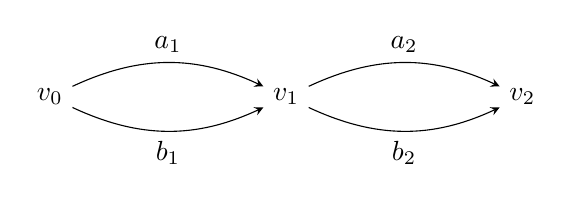
\begin{tikzpicture}[>=stealth]
\node (v0) at(0,0){$v_0$};\node(v1)at(3,0){$v_1$};\node(v2)at(6,0){$v_2$};
\draw[->](v0)to[bend left=25]node[above]{$a_1$}(v1);\draw[->](v0)to[bend right=25]node[below]{$b_1$}(v1);
\draw[->](v1)to[bend left=25]node[above]{$a_2$}(v2);\draw[->](v1)to[bend right=25]node[below]{$b_2$}(v2);
\end{tikzpicture}\par Figure 1. $2$-garland.\end{center}
Let $G:=(V,E)$ be a directed graph. Each edge $e\in E$ has the corresponding variable $x_e$, where $x_e=1$ indicates that a flow of size $1$ is going through an edge $e$. Let $u$ be an arbitrary, but fixed vertex of the graph.
The formula $\Flow_{G,u}$ consists of the following constraints written in CNF for all $v\in V$:
\[\sum_{e\in E:\st(e)=v}x_e-\sum_{e\in E:\en(e)=v}x_e\ge c(v),\]
where $e=(\st(e),\en(e))$ and $c:V\to\{0,1\}$ is a labeling function:
\[c(v)=0,\text{ for all }v\in V\setminus\{u\};\qquad c(u)=1.\]
This formulas states: for all vertices in the graph the flow is non-negative, and at least for one vertex it is strictly positive. It is easy to see that $\Flow_{G,u}$ is unsatisfiable. We omit index $u$ since in our applications it is an arbitrary vertex.
We use the most naive CNF encoding of these constraints. We represent each constraint separately. Consider a vertex $v\in V$ and a set of edges $E_v:=\{e_1,e_2,\ldots,e_s\}\subseteq E$ that are incident to $v$. Let $\rho_v:E_v\to\{0,1\}$ be an assignment that violates the constraint in $v$. In this case we add to the formula a clause $C$:
\[x_{e_1}^{1-\rho(x_{e_1})}\vee x_{e_2}^{1-\rho(x_{e_2})}\vee\cdots\vee x_{e_s}^{1-\rho(x_{e_s})},\]
and we also say that this assignment has a gap:
\[g(\rho_v):=c(v)-\sum_{e\in E:\st(e)=v}\rho_v(x_e)+\sum_{e\in E:\en(e)=v}\rho_v(x_e).\]
For our purpose we consider $\Flow_G$ based on expanders. To be precise, we start with a graph $G$ that is an $(n,\Delta,\alpha)$-expander, where $\Delta=\Theta(\log n)$ and $\alpha$ is some fixed constant, and replace each undirected edge by two directed edges (we say that these edges are dual). The exact value of $\Delta$ depends on a value of $k$.
\begin{result}{Remark 15}
We consider only proper partial assignments $\rho$ that satisfy the following property for all pairs of dual edges $(e,e')$:
\begin{itemize}\item $\rho(x_e)\in\{0,1\}$ iff $\rho(x_{e'})\in\{0,1\}$;
\item if $\rho(x_e)=1$ then $\rho(x_{e'})=0$.\end{itemize}
We also identify $\supp(\rho)$ with an undirected set of edges that are assigned by $\rho$.
\end{result}
To make the formula somewhat ``confusing'' for $(1,+k)$-BP, we would like to add more variables to clauses. These variables do not really affect the physical meaning of the formula, but make it hard for $(1,+k)$-BP to extract additional information from repetitions on paths. This transformation is sensitive to the exact CNF encoding of the constraints that is written above.
\begin{result}{Definition 16}
Let $G:=(V,E)$ be an undirected graph and $C_v$ be a subset of clauses corresponding to vertex $v$ in $\Flow_G$. Let $\eta_v^k:C_v\to\binom{E}{k}$ be a mapping, and $\eta^k:=\{\eta_v^k\mid v\in V\}$ be a family of such mappings. We define $\Flow_G^{\eta^k}$ the following way:
\begin{itemize}\item for each $v\in V$ we consider each $C\in C_v$;
\item we take $\eta_v^k(C)=\{e_1,\ldots,e_k\}$, which is a set of $k$ edges;
\item we replace $C$ by $2^{2k}$ clauses of the form:
\[C\vee\bigvee_i x_{s_i}^{a_i}\vee x_{s'_i}^{a'_i}\]
enumerated by $a_i,a'_i\in\{0,1\}$, where $i\in[k]$ and $s_i,s'_i$ are directed copies of the edge $e_i$.\end{itemize}
\end{result}
As described in the plan, at some point in the proof we would like to construct an assignment that leaves certain clauses (to which a certain set of variables was added) unsatisfied. For our purpose, we would like those clauses to ``strongly unsatisfy'' the condition in their vertices.
Let us describe the construction of $\eta^k$. Assume that $\Delta\ge50\cdot k\log n$. For each $v\in V$ we define $\eta_v$ independently. We will be interested in adding variables to clauses which correspond to large incoming flow.
\begin{enumerate}
\item Let us consider a set of clauses $\mathcal C$ that corresponds to $v$ and a proper partial assignment on edges incident to $v$ with gap equal to $\Delta/4+1$.
\item Note that $|\mathcal C|\ge\binom{\Delta}{\Delta/4}\ge4^{\Delta/4}\ge n^{4k}$. The first inequality holds since we can choose arbitrary $\Delta/4+1$ incoming edges to obtain the desired gap and set all other incident edges to zero.
\item There are at most $\binom{n\Delta}{k}\le(n\Delta e/k)^k\le n^{2k}$ different sets of $k$ edges. Hence we can choose a subset of $B\subseteq\mathcal C$ and define $\eta_v^k$ to be a bijection between $B$ and all possible choices of sets of $k$ edges.
\end{enumerate}
Note that the existence of $(1,+k)$-BP of size $S$ solving $\Search_{\Flow_G^{\eta^k}}$ (for any $\eta^k$) implies the existence of $(1,+k)$-BP of size $S$ solving $\Search_{\Flow_G}$.
\subsection*{4.1.1 Locally Consistent Assignments}
We need a notion of ``good assignments'', i.e. assignments that reduce $\Flow_G$ formulas to smaller, but ``equally hard'' instances.
Let $G:=(V,E)$ be a graph. A proper assignment $\rho$ $\delta$-satisfies a set of vertices $U\subseteq V$ iff for all $v\in U$ the following holds:
\begin{itemize}\item $\rho$ assigns all edges that are incident to $v$;
\item $\rho$ satisfies the constraint for $v$;
\item $\sum_{e\in E:\st(e)=v}\rho(x_e)\ge\delta\cdot\Delta$.\end{itemize}
We also say that a proper assignment $\rho$ is $(r,\delta,\beta)$-locally consistent iff there is a set of vertices $V_\rho$ of size at most $r$ such that:
\begin{itemize}\item $\rho$ $\delta$-satisfies $V_\rho$;
\item $(V\setminus V_\rho,E\setminus\supp(\rho))$ satisfies $(r,\beta)$-expansion property.\end{itemize}
\begin{result}{Remark 17}
If $\rho$ is an $(r,\delta,\beta)$-locally consistent assignment for some $\beta>0$, then $V_\rho$ is uniquely defined.
\end{result}
\begin{proof}
For the sake of contradiction assume that there are two candidates $A,B$. Wlog $A\setminus B\ne\emptyset$. Pick an arbitrary vertex $v\in A\setminus B$. Since $A$ satisfies the required properties, $\rho$ assigns all edges that are incident to $v$, which contradicts the fact that $(V\setminus B,E\setminus\supp(\rho))$ satisfies $(r,\beta)$-expansion property.
\end{proof}
\section*{Original Section 4.2: Proof of Theorem 2 (p.17:10)}
Let $G$ be an $(n,\Delta,\alpha)$-expander and $\eta^{k_0+1}$ be a mapping defined in section 4.1. In this section we prove an exponential lower bound on $\Search_{\Flow_G^{\eta^{k_0+1}}}$ for $(1,+k_0)$-BP. We assume that $n$ is large enough.
Let us fix some parameters:
\begin{itemize}
\item $\Delta:=100k_0\log n$ and $\Delta>200$;
\item $\alpha:=0.01$ is the second eigenvalue of the normalized adjacency matrix of $G$;
\item $r:=n/\Delta$ and $\beta:=0.96$ is the ``combinatorial expansion'' of the graph $G$;
\item $\beta':=0.95$ is an expansion parameter that we try to maintain after removing some vertices and edges from $G$;
\item $\nu_k:=(\tfrac14(\beta-\beta'))^{k+3}$ is a scaling factor that indicates the fraction of edges that we want to assign in our partial assignment.
\end{itemize}
Note that $r\ll(1-\beta-\alpha)n=0.03\cdot n$ and hence by Corollary 11 $G$ satisfies $(r,\beta)$-expansion property, hence we can use all combinatorial expansion properties and tools.
To formulate the induction hypothesis we need one more definition. Let $M\subseteq E$ and $\rho$ is a proper assignment. We say that $\rho$ is $\gamma$-minimal local consistent extension or (mlce) on $M$ iff:
\begin{itemize}\item $\rho$ is $(r,0.6,\gamma)$-locally consistent assignment;
\item $\supp(\rho)=M\cup E(V_\rho)$;
\item $|E(V_\rho,\overline{V_\rho})\setminus M|<\gamma\Delta|V_\rho|$.\end{itemize}
Informally we may think about it in the following way: after we assign edges from $M$ somehow, $\rho$ should assign also $V_\rho$ as a ``minimal'' set of vertices to take care of in order to be locally consistent.
Let $\varphi:=\Flow_G^{\eta^{k_0+1}}$. By induction on $k\le k_0$ we show the following statement. For all sets of edges $M\subseteq E$ of size at most $\nu_k\Delta r$ and all $\beta'$-mlce $\rho$ on $M$ any $(1,+k)$-BP for $\Search_{\varphi|_\rho}$ has size at least $2^{\frac{\nu_k}{4(k+1)^2}\Delta r}$.
Fix some $M,\rho,0\le k\le k_0$ and for the sake of contradiction assume that we have a $(1,+k)$-BP $D$ of size $2^{\frac{\nu_k}{4(k+1)^2}\Delta r}$ for $\Search_{\varphi|_\rho}$.
